\documentclass[a4paper,12pt]{article}
\usepackage[utf8]{inputenc}
\usepackage{geometry}
\usepackage{longtable}
\usepackage{booktabs}
\usepackage{array}
\usepackage{graphicx}
\usepackage{tikz}
\usepackage{hyperref}
\usepackage{amsmath}
\usepackage{caption}
\usepackage{xcolor}

% Page Setup
\geometry{a4paper, margin=1in}
\hypersetup{
    colorlinks=true,
    linkcolor=blue,
    filecolor=magenta,
    urlcolor=cyan,
}

% Title and Metadata
\title{\textbf{Professional Black-Box Testing Plan for NVD API Integration}}
\author{Prepared by: [Your Name]}
\date{\today}

\begin{document}

\maketitle

\section*{Introduction}
This document outlines a rigorous black-box testing plan for the NVD API integration, adhering strictly to ISTQB standards. The plan utilizes **Equivalence Partitioning**, **Boundary Value Analysis**, **Decision Tables**, and **State Transition Diagrams** to ensure comprehensive testing without accessing internal implementation details.

\newpage
\section*{1. Equivalence Partitioning Analysis}
Equivalence Partitioning (EP) divides inputs into valid and invalid partitions to ensure comprehensive coverage with minimal test cases.

\subsection*{Test Cases}
\begin{longtable}{|p{2cm}|p{5cm}|p{4cm}|p{4cm}|}
\hline
\textbf{Partition ID} & \textbf{Partition Description} & \textbf{Sample Input} & \textbf{Expected Result} \\
\hline
EP-01 & Valid Keywords & \texttt{java} & API returns CVE data \\
\hline
EP-02 & Invalid Keywords (Special Characters) & \texttt{\%\$\#} & API returns empty or error response \\
\hline
EP-03 & No Input (Empty Query) & None & Returns default error or missing keyword message \\
\hline
EP-04 & Valid API Key & \texttt{validKey123} & API responds with status 200 \\
\hline
EP-05 & Invalid API Key & \texttt{invalidKey} & API responds with status 401 and "Unauthorized" \\
\hline
\end{longtable}

\newpage
\section*{2. Boundary Value Analysis}
Boundary Value Analysis (BVA) focuses on testing the edge values of valid and invalid input ranges.

\subsection*{Boundary Cases for Pagination Parameters}
\begin{longtable}{|p{2cm}|p{6cm}|p{4cm}|p{3cm}|}
\hline
\textbf{Test Case ID} & \textbf{Description} & \textbf{Input} & \textbf{Expected Result} \\
\hline
BVA-01 & Minimum valid offset and limit & Offset: 0, Limit: 1 & Returns 1 CVE item \\
\hline
BVA-02 & Maximum valid limit & Offset: 0, Limit: 100 & Returns 100 CVE items \\
\hline
BVA-03 & Below minimum limit & Offset: 0, Limit: 0 & Status 400, "Invalid limit" \\
\hline
BVA-04 & Above maximum limit & Offset: 0, Limit: 101 & Status 400, "Limit exceeded" \\
\hline
BVA-05 & Large offset value & Offset: 5000, Limit: 10 & API handles request without performance degradation \\
\hline
\end{longtable}

\section*{3. Decision Table Analysis}
Decision Tables are used to test complex combinations of conditions and actions.

\subsection*{Decision Table for API Authorization and Keyword Search}
\begin{longtable}{|c|c|c|c|c|}
\hline
\textbf{Condition 1} & \textbf{Condition 2} & \textbf{Condition 3} & \textbf{Action} & \textbf{Expected Output} \\
\hline
Valid API Key & Valid Keyword & Correct Pagination & Perform Search & Status 200, CVE data returned \\
\hline
Valid API Key & Invalid Keyword & Correct Pagination & Perform Search & Status 200, empty response \\
\hline
Invalid API Key & Any Keyword & Any Parameters & Deny Access & Status 401, "Unauthorized" \\
\hline
Valid API Key & Valid Keyword & Incorrect Pagination & Reject Request & Status 400, "Invalid parameters" \\
\hline
\end{longtable}

\section*{4. State Transition Diagram}
State Transition Diagrams model the dynamic behavior of the API based on input-triggered state changes.

\begin{figure}[h!]
    \centering
    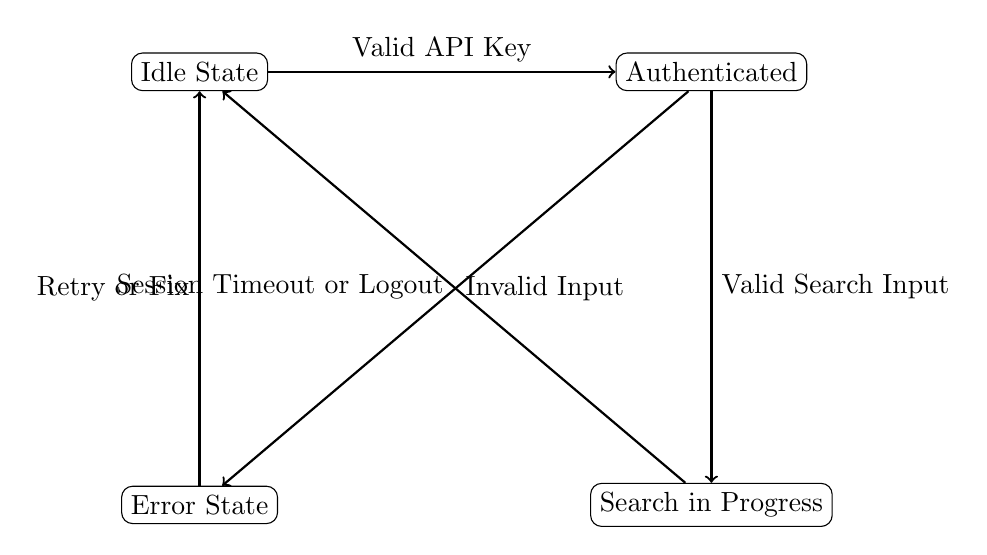
\begin{tikzpicture}[node distance=2.5cm, auto]
        % Nodes
        \node[draw, rectangle, rounded corners] (Idle) {Idle State};
        \node[draw, rectangle, rounded corners, right of=Idle, xshift=4cm] (Auth) {Authenticated};
        \node[draw, rectangle, rounded corners, below of=Auth, yshift=-3cm] (Search) {Search in Progress};
        \node[draw, rectangle, rounded corners, left of=Search, xshift=-4cm] (Error) {Error State};

        % Arrows
        \draw[->, thick] (Idle) -- node[midway, above] {Valid API Key} (Auth);
        \draw[->, thick] (Auth) -- node[midway, right] {Valid Search Input} (Search);
        \draw[->, thick] (Auth) -- node[midway, right] {Invalid Input} (Error);
        \draw[->, thick] (Search) -- node[midway, left] {Session Timeout or Logout} (Idle);
        \draw[->, thick] (Error) -- node[midway, left] {Retry or Fix} (Idle);
    \end{tikzpicture}
    \caption{State Transition Diagram for NVD API Workflow}
    \label{fig:state-transition}
\end{figure}

\newpage
\section*{5. Critical Observations and Gaps}
\begin{itemize}
    \item \textbf{API Usability}: Error messages must clearly describe issues (e.g., invalid parameters or keys).
    \item \textbf{Performance under Load}: Large offset and limit combinations must be stress-tested.
    \item \textbf{Security Robustness}: SQL injection or malformed inputs must be gracefully handled.
    \item \textbf{State Handling}: The API must return to the idle state after an error or successful operation.
\end{itemize}

\section*{Conclusion}
This black-box testing plan rigorously validates the NVD API using:
\begin{itemize}
    \item **Equivalence Partitioning**: Simplifies testing by dividing inputs into logical partitions.
    \item **Boundary Value Analysis**: Ensures robust handling of edge cases.
    \item **Decision Tables**: Covers all possible input combinations and outputs.
    \item **State Transition Diagrams**: Models the API’s dynamic behavior under various scenarios.
\end{itemize}

By adhering to ISTQB principles, this plan ensures functional, secure, and reliable API performance while maintaining compliance with industry standards.

\end{document}
